% !TEX root = ../notes_template.tex
\chapter{Muscle Regulation}\label{chp:regulation}
Updated on \today
\minitoc

This chapter introduces the mechanisms utilized by the central nervous system (CNS) to regulate active tension. To regulate active tension means to vary its force from its lowest value (resting tone) to its maximal value (maximal voluntary contraction (MVC)). Active tension is developed at the level of the sarcomere, excitation at the level of the muscle fiber, regulation occurs at the level of motor units. A motor unit includes an $\alpha$-motor neuron and all of the muscle fibers it innervates. The CNS has two strategies to regulate active tension. One strategy is to manipulate the number of twitches per second (frequency summation or rate coding); and the second strategy is to manipulate the number of motor units twitching (motor unit summation or motor unit recruitment). Between these two approaches there is a nearly continuous variation in active tension possible, with some muscles (fine motor) having a greater capacity for continuous variation than others (gross motor).

\vspace{5mm}

\textbf{Objectives include:}
\begin{enumerate}
    \item Explain motor unit structure–function relationships.
    \item Explain muscle fiber differentiation (types) structure-function relationships.
    \item Explain motor unit excitation, twitch and tetany.
    \item Compare and contrast frequency summation (rate coding) and motor unit summation (recruitment).
    \item Explain the order of recruitment.
    \item Explain how the muscle spindles and the golgi tendon organs influence motor unit excitation.
    \item Explain the physiological basis of the electromyogram (EMG) and limitations of EMG interpretation.
    \item Explain the effect of amyotrophic lateral sclerosis and aging on motor units.
    \item Explain the effect of peripheral nerve demyelination on muscle regulation.
\end{enumerate}\

\section{Motor Units}

A motor unit is an $\alpha$-motor neuron and all of muscle fibers that its terminal axon branches form a neuromuscular junction at a motor end plate. Each muscle fiber has one motor end plate, and therefore one neuromuscular junction. However, each $\alpha$-motor neuron has many terminal axon branches. The muscle fibers of a single motor unit are randomly dispersed throughout the muscle epimysium. Therefore, the muscle fibers of a motor unit contribute to the tension developed in several fascicles. This arrangement ensures that when only a few motor units are excited there are muscle fibers throughout the entire muscle generating tension at the tendon attachments to avoid asymmetrical pull from one fascicle or isolated location within the epimysium.

\begin{figure}[!ht]
    \centering
    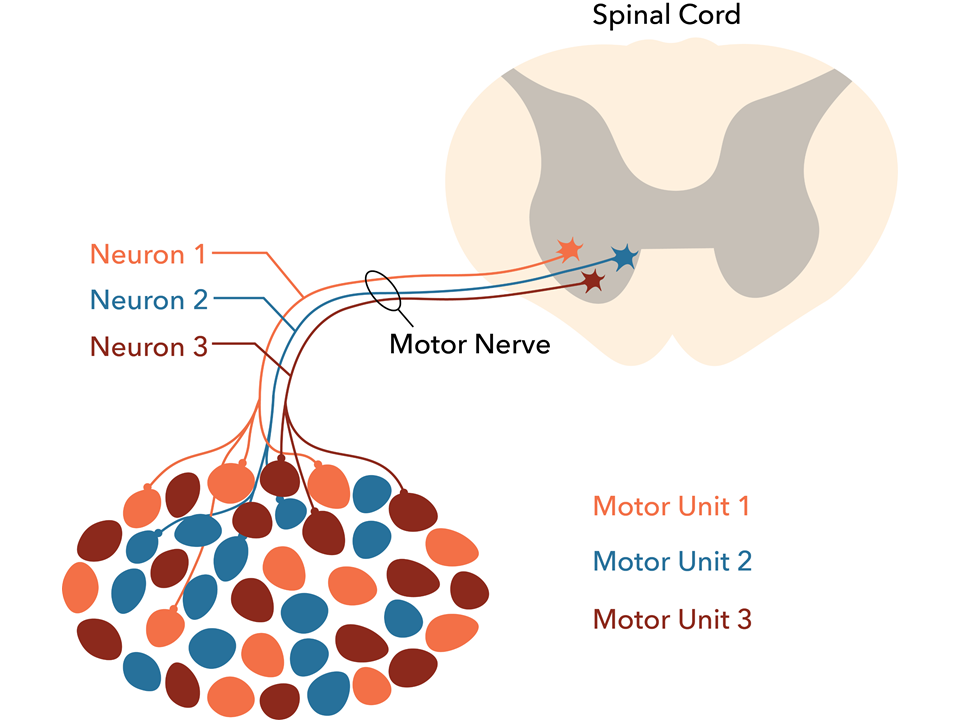
\includegraphics[width=1\linewidth]{./figure/motor_unit.png}
    \caption{Motor Unit Distribution in a Muscle \footnotesize{\href{https://commons.wikimedia.org/wiki/File:Motor_unit.png}{Wikimedia Commons, CC BY 4.0})}}
    \label{fig:motor_unit}
\end{figure}

\subsection{Innervation Ratio}
Motor unit innervation ratio (IR) refers to the number of muscle fibers per motor unit and is usually given as the average number of muscle fibers per motor unit.

\begin{equation}
    IR = \frac{N_{mf}}{N_{mu}}
\end{equation}

The IR varies between muscles and differentiates muscles equipped for fine or gross motor control (See Table \ref{table:Innervation_Ratios}). IRs vary from 5 in muscles in the eye (i.e. lateral rectus) to approximately 1700 in muscles in the calf for locomotion (i.e. gastrocnemius).

\begin{table}[h!]
\centering
\begin{tabular}{||c c c c||} 
 \hline
 Muscle & $\alpha$-motor neurons & Muscle Fibers ($\times 10^3$) & Innervation Ratio \\ [0.5ex] 
 \hline\hline
 Lateral Rectus (eye) & 30* &.15* & 5 \\
 Lumbricals (hand) &  98 & 10.3 & 105 \\ 
 Brachialis & 330 & 130 & 393 \\
 Biceps  & 774 & 580 & 749 \\ 
 Gastrocnemius & 580 & 1000 & 1724 \\[1ex] 
 \hline
\end{tabular}
\caption{Variability of Innervation Ratio in Human Muscles (\footnotesize{From \cite{buchthal_motor_1980}, (* Estimates that need confirmation)})}
\label{table:Innervation_Ratios}
\end{table}

IRs for whole muscles are explanatory for the concept of fine motor and gross motor control. Considering tension is developed by muscle fibers, the number of muscle fibers recruited with each new motor unit recruited influences the size of jumps in active tension. Muscles with lower IRs have greater regulation (control) over the amount of tension they produce because they better accommodate continuous increments in tension with each new motor unit recruited. Of five muscles in Table \ref{table:Innervation_Ratios}, the lateral rectus (eye) and lumbricals (muscle in the hand) have the greatest fine motor control. While the gastrocnemius is responsible for the greatest need for high tension (force) output (gross motor control).

\subsection{Motor Unit \& Muscle Fiber Types}

While IRs for whole muscles help explain variation between muscles with differences in motor control they ignore the systematic variation in the number of muscle fibers per motor unit within a muscle. There are different types of motor units. The types include differences in the $\alpha$-motor neurons, the muscle fibers and the IR. The differences are structural and functional. Types exist on a spectrum with transitions in many (but not all) of the characteristics between them. Despite the spectrum, and using different characteristics, experts have identified and agree on classification systems that converge on three types of human motor units and associated muscle fibers \cite{lieber_skeletal_2010}.

\begin{itemize}
    \item Fast Fatigable (FF) Motor Units with Fast Glycolytic (FG) (Type 2a) Muscle Fibers
    \item Fast Resistant (FR) Motor Units with Fast Oxidative (FOG) (Type 2x) Muscle Fibers
    \item Slow (S) Motor Units with Slow Oxidative (SO) (Type 1) Muscle Fibers
\end{itemize}

The above classification names are all utilized, however the Type 1, 2x and 2a are probably the most common. The other classifications are informative about the functional characteristics of the motor units and muscle fibers they innervate. Beyond their coherence, the motor unit classifications FF, FR and S share a feature with the muscle fiber classifications FG, FOG and SO. They both use the letters F and S to represent Fast and Slow, and they primarily refer to faster or slower excitation (and in the case of muscle fibers also activation). 

The second letter F in FF, and the letters R and S (dual use of the meaning slow for the Slow motor units), and the letters G and O for muscle fibers are related to functional characteristics of fatigue and energetics. For motor unit classifications the second F in FF stands for fatigable, meaning FF fibers are fatigable and cannot sustain tetany for very long. The R in FR motor units stands for resistant, as in fatigue resistant. They resist (for a time) the fatigue of FF motor units. And the S motor units are slow, both in excitation, and slow to fatigue (hence the "dual use" of slow). In Chapter \ref{chp:energetics} on Energetics, the concept of fatigue denoted in muscle fiber classification letters G and O refer to the biochemical pathways that produce ATP, glycolosis and oxidative (including both the citric acid (Kreb's) cycle and electron transport). The connection between FF and FG, FR and FOG, and S with SO, has to do with the rate and sustainability of ATP production by these pathways. Glycolosis has a relatively high rate and low sustainability, and oxidative pathways have a relatively low rate and high sustainability. These pathways, but not just these pathways, result in the fatigability, fatigue resistant or slow to fatigue characterizations of motor units and their fibers. While fatigability comes up in this chapter, the focus is on the excitation and activation characteristics of the fast and slow motor units and muscle fibers.

\subsubsection{Fast vs. Slow - An excitable concept}

The terms fast and slow refer to relative differences in functional characteristics between $\alpha$-motor neuron and the muscle fibers. The functional characteristics fast and slow are associated with a set of functionally coherent structural differences. The section below focuses on the most distinguishing structural characteristics that influence the functional characteristics of excitation and activation.

\paragraph{Fast \& Slow $\alpha$-Motor Neurons}
Fast and slow for the motor unit $\alpha$-motor neuron refers to how quickly excitations can be sent which influences how frequently they can be excited. The faster an excitation propagates down an axon the sooner it is ready for another excitation. In a sequence of excitations, if a second excitation catches up to the first excitation it will cease propagation once it reaches a section of the axon membrane that is its refractory period from the first excitation. A fast neuron has a higher nerve conduction velocity (NCV) and a higher maximum excitation frequency (Hz) than a slow neuron.

NCV is related to the size of the neuron (diameter) because diameter influences resistance to current. Current is the flow (flow is a rate) of electrical impulses and therefore directly related to velocity. Diameter is inversely proportional to resistance, and resistance is inversely proportional to current, therefore diameter is directly proportional to current and velocity (See Figure \ref{fig:Current_Resistance}). The large diameter of the $\alpha$-motor neurons, combined with the myelin sheaths (The role of myelin was introduced in Chapter \ref{chp:excitation}), contribute to its relatively high NCV. 

\begin{figure}[!ht]
    \centering
    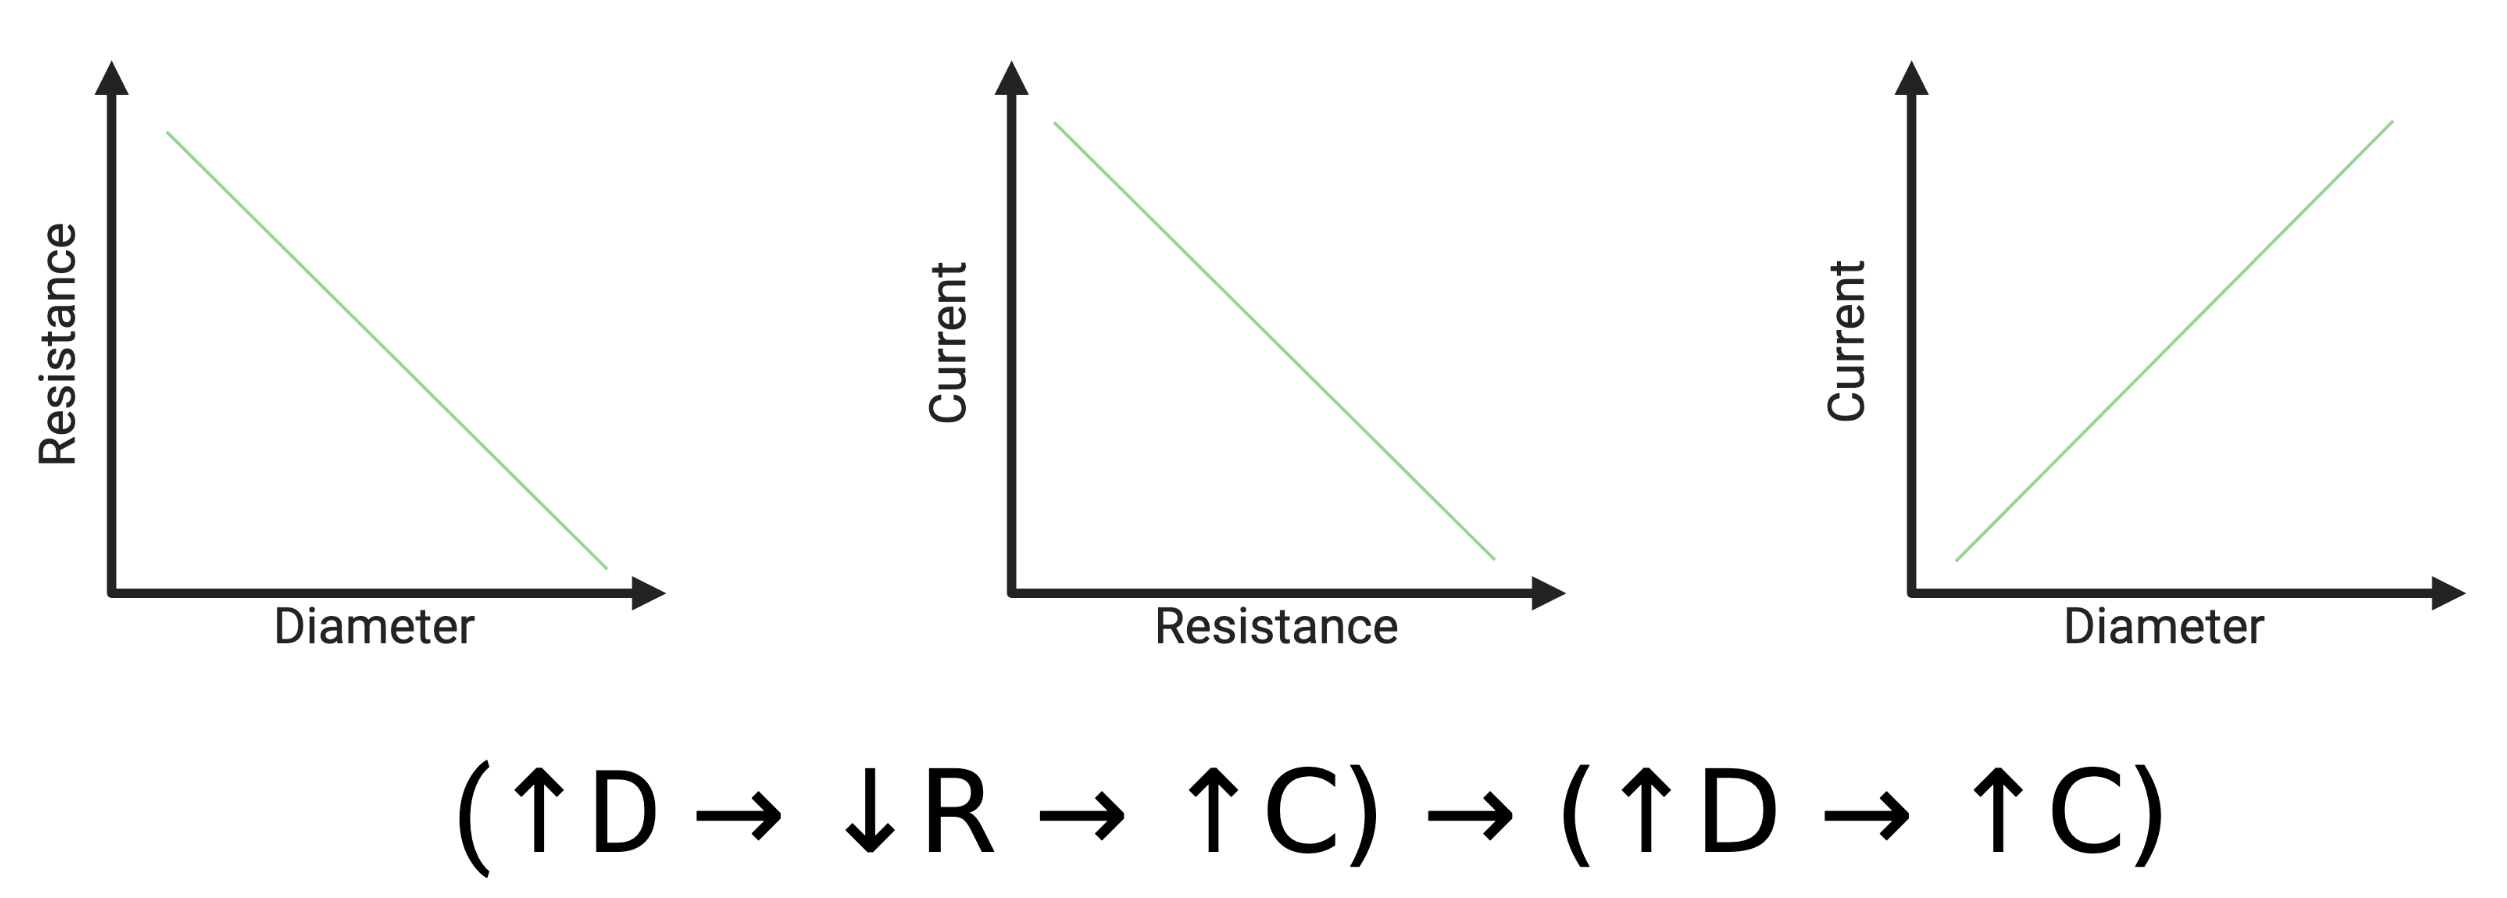
\includegraphics[width=1\linewidth]{./figure/Current_Resistance.png}
    \caption{Relationship between Diameter, Resistance and Current \footnotesize{(Created in BioRender.com)}}
    \label{fig:Current_Resistance}
\end{figure}

Estimated NCVs for three nerve fiber types are presented in Table \ref{table:NCV}. The $\alpha$-motor neuron has the highest NCV. The variation in diameter in the $\alpha$-motor neuron is explained by the motor unit types with the fast (FF) motor units innervating the FG fibers having the larger diameter ($\simeq 22 \mu m$) on the higher end for NCV ($\simeq 120 m \cdot s^{-1}$), and the S motor units with the small diameters ($\simeq 12 \mu m$)and the lower end of NCV ($\simeq 70 m \cdot s^{-1}$) (and FR motor units innervating FOG somewhere in the middle).  The terms fast and slow for the $\alpha$-motor neurons of motor units are relative to one another. It is clear in Table \ref{table:Innervation_Ratios} that both fast and slow $\alpha$-motor neurons are faster than the other neurons listed. They are faster due to both diameter (as compared to $\delta$-sensory neurons) and additionally myelination (as compared to C sensory neurons).

\begin{table}[h!]
\centering
\begin{tabular}{||c c c c ||} 
 \hline
Nerve Fiber & Diameter (\mu m) & NCV ($m \cdot s^{-1}$) & Function \\ 
 \hline\hline
 $\alpha$-motor & 12-22 & 70-120 & motor \\ 
 $\delta$-sensory & 1-5 & 12-30 & sharp pain \\
 C & 0.5-1.2 & 0.2-2 & dull pain \\ [1ex] 
 \hline
\end{tabular}
\caption{NCV for different nerve fiber types. Note: C fibers are unmyelinated, whereas $\alpha$-motor and $\delta$-sensory fibers are myelinated. Therefore, C fibers have a larger drop in NCV than would be estimated just from diameter. \footnotesize{Data from \cite{feher_quantitative_2017}}}
\label{table:NCV}
\end{table}

A fast $\alpha$-motor neuron has a larger diameter and myelin (structure) which both contribute to the NCV (function). Since the neurons of slow motor units are also myelinated the primary structural differentiation between fast and slow motor unit neurons are their size (larger diameters in fast motor unit neurons). Structurally, these larger neurons also innervate a higher number of muscle fibers. In mammalian muscles the IR for FF motor units is approximately twice (2x) that of S motor units, but this is an estimate that varies considerably between muscles (range from 1.1x to 3x greater than S motor units) \cite{bodine_maximal_1987}. 

A consequence of a larger neuron is that it requires more CNS excitation to become excited (excitation inertia). Excitation inertia has to do with how many ligand voltage gated channels must be opened before the threshold potential is reached. The larger (and thus faster) neuron has more excitation inertia. Fast $\alpha$-motor neurons are larger. While fast, they take more excitation to be excited. This is an important feature for motor unit recruitment and the size principle of recruitment order covered later in the chapter.

\paragraph{A note on motor unit and muscle fiber integrity}
Fast (larger) and slow (smaller) $\alpha$-motor neurons play a role for motor unit and muscle fiber integrity. The narrative of this chapter is that there is coherence between the neuron doing the excitation, and the muscle fibers being excited so that they can be activated. The neuron excitations play a critical, causal, role in determining the type of muscle fiber \cite{buchthal_motor_1980}. It is not a coincidence that faster and larger motor neurons innervate faster and larger muscle fibers. Studies using electrical stimulation and crossover (changing which neurons innervate which muscles), many muscle fiber characteristics change from slow to fast or from fast to slow. These experiments conclude that there is plasticity at the level of muscle fiber type with such experimental manipulations, and that this plasticity is related to the differences in electrical (not chemical) stimulus. The challenge to anyone wishing to alter their fiber type dominance is finding a way to  tap into the plasticity of the neurons.\footnotemark\footnotetext{Certain characteristics such as myosin and myosin ATPase isoforms rely on gene expression (one isoform is expressed or the other is expressed) and therefore may provide a limit to how much, or how many, muscle fibers have this plasticity.}

\paragraph{Summary of Fast \& Slow $\alpha$-Motor Neurons}
The functional characteristics that make the fast $\alpha$-motor neuron of the fast motor unit fast as compared to the slow classification are a higher NCV and a higher excitation frequency. The predominant structural difference that leads to these functional differences is the size of the neuron (larger, larger diameter). These structural and resultant functional differences fit on a spectrum that, in Table \ref{table:NCV}, result in a wide range of neuron diameters. These neuronal excitation characteristics innervate, and actually contribute to, coherence between the neuron and the muscle fibers of the motor unit.


\paragraph{Fast \& Slow Muscle Fibers}

The functional characteristics of muscle fibers that make them fast vs. slow include both structures related to excitation-activation coupling as well as structures related to activation (crossbridge kinetics). 

For muscle fibers in a fast motor unit to respond to the faster and higher excitation frequency of the neurons they require a well developed T-tubule and sarcoplasmic reticulum (SR) system. The SR and T-system of fast fibers can have up to three times the volume of slow fibers. This allows fast motor units to convert the higher frequency of nerve excitation into a higher frequency of muscle fiber activation.

With a higher frequency of muscle fiber activation there must be structural changes that also allow for faster crossbridge kinetics, otherwise the faster activation (faster release and update of $Ca^{2+}$ for example) would not result in faster twitches. The crossbridge kinetic structural changes tend to be discrete rather than on a spectrum.\footnotemark\footnotetext{By discrete we mean that there are no intermediate or transition steps between the structure. This is compared to changes such as the size of a SR or the diameter of a neuron or the number of ACh receptors at a NMJ where there can any number of transitional steps.} Fast fibers express an isoform of the protein myosin (particularly the heavy chain) and the enzyme (also a protein) myosin ATPase (responsible for hydrolyzing ATP on the myosin head). The combination of these two expressions allow for faster crossbridge kinetics (cycling through the sliding filament model) which leads to slightly more tension at the level of the sarcomere and a higher velocity for shortening \cite{larsson_maximum_1993, schiaffino_molecular_1996}. Therefore, when isolated or when either of these types of fibers dominate in a particular muscle, the force-velocity curve is shifted upward in fast as compared to slow motor units, with fast (FF) motor units having a higher velocity for any given force, and a higher force for any given velocity. 

These differences result in higher specific tension ($T_s$) in fast muscle fibers. $T_s$ refers to the tension developed per sarcomere or, more commonly considered, tension developed per unit of cross-sectional area. Since there are more muscle fibers in fast motor units means there are more sarcomeres and a greater cross sectional area, the $T_s$ makes the tension of a motor unit relative to its cross sectional area to allow comparison that avoids the confounding effect of greater cross sectional area.

The molecular (signal transduction) events that lead to the expression of myosin and myosin ATPase isoforms have not yet been completely uncovered.\footnotemark\footnotetext{Though, the author (SC) is still reading about the possibilities.} It is assumed that, due to the plasticity of muscle fiber types reported in experimental conditions, at least some muscle fibers retain the ability to express either isoform and that there exists a molecular mechanism that can theoretically be switched \cite{schiaffino_molecular_1996}.

\paragraph{Summary of Fast \& Slow Muscle Fibers}
The functional characteristics of muscle fibers for fast motor units allow for faster excitation-activation coupling and faster crossbridge kinetics. The structural characteristics that enable these include a higher volume of T-tubules and SR (for activation) and an isoform of myosin and myosin ATPase (for crossbridge kinetics). These changes result in an upward shifted force-velocity curve for fast motor units as compared to slow motor units (Figure \ref{fig:fiber_type_FV}). 

\begin{figure}[h]
    \centering
    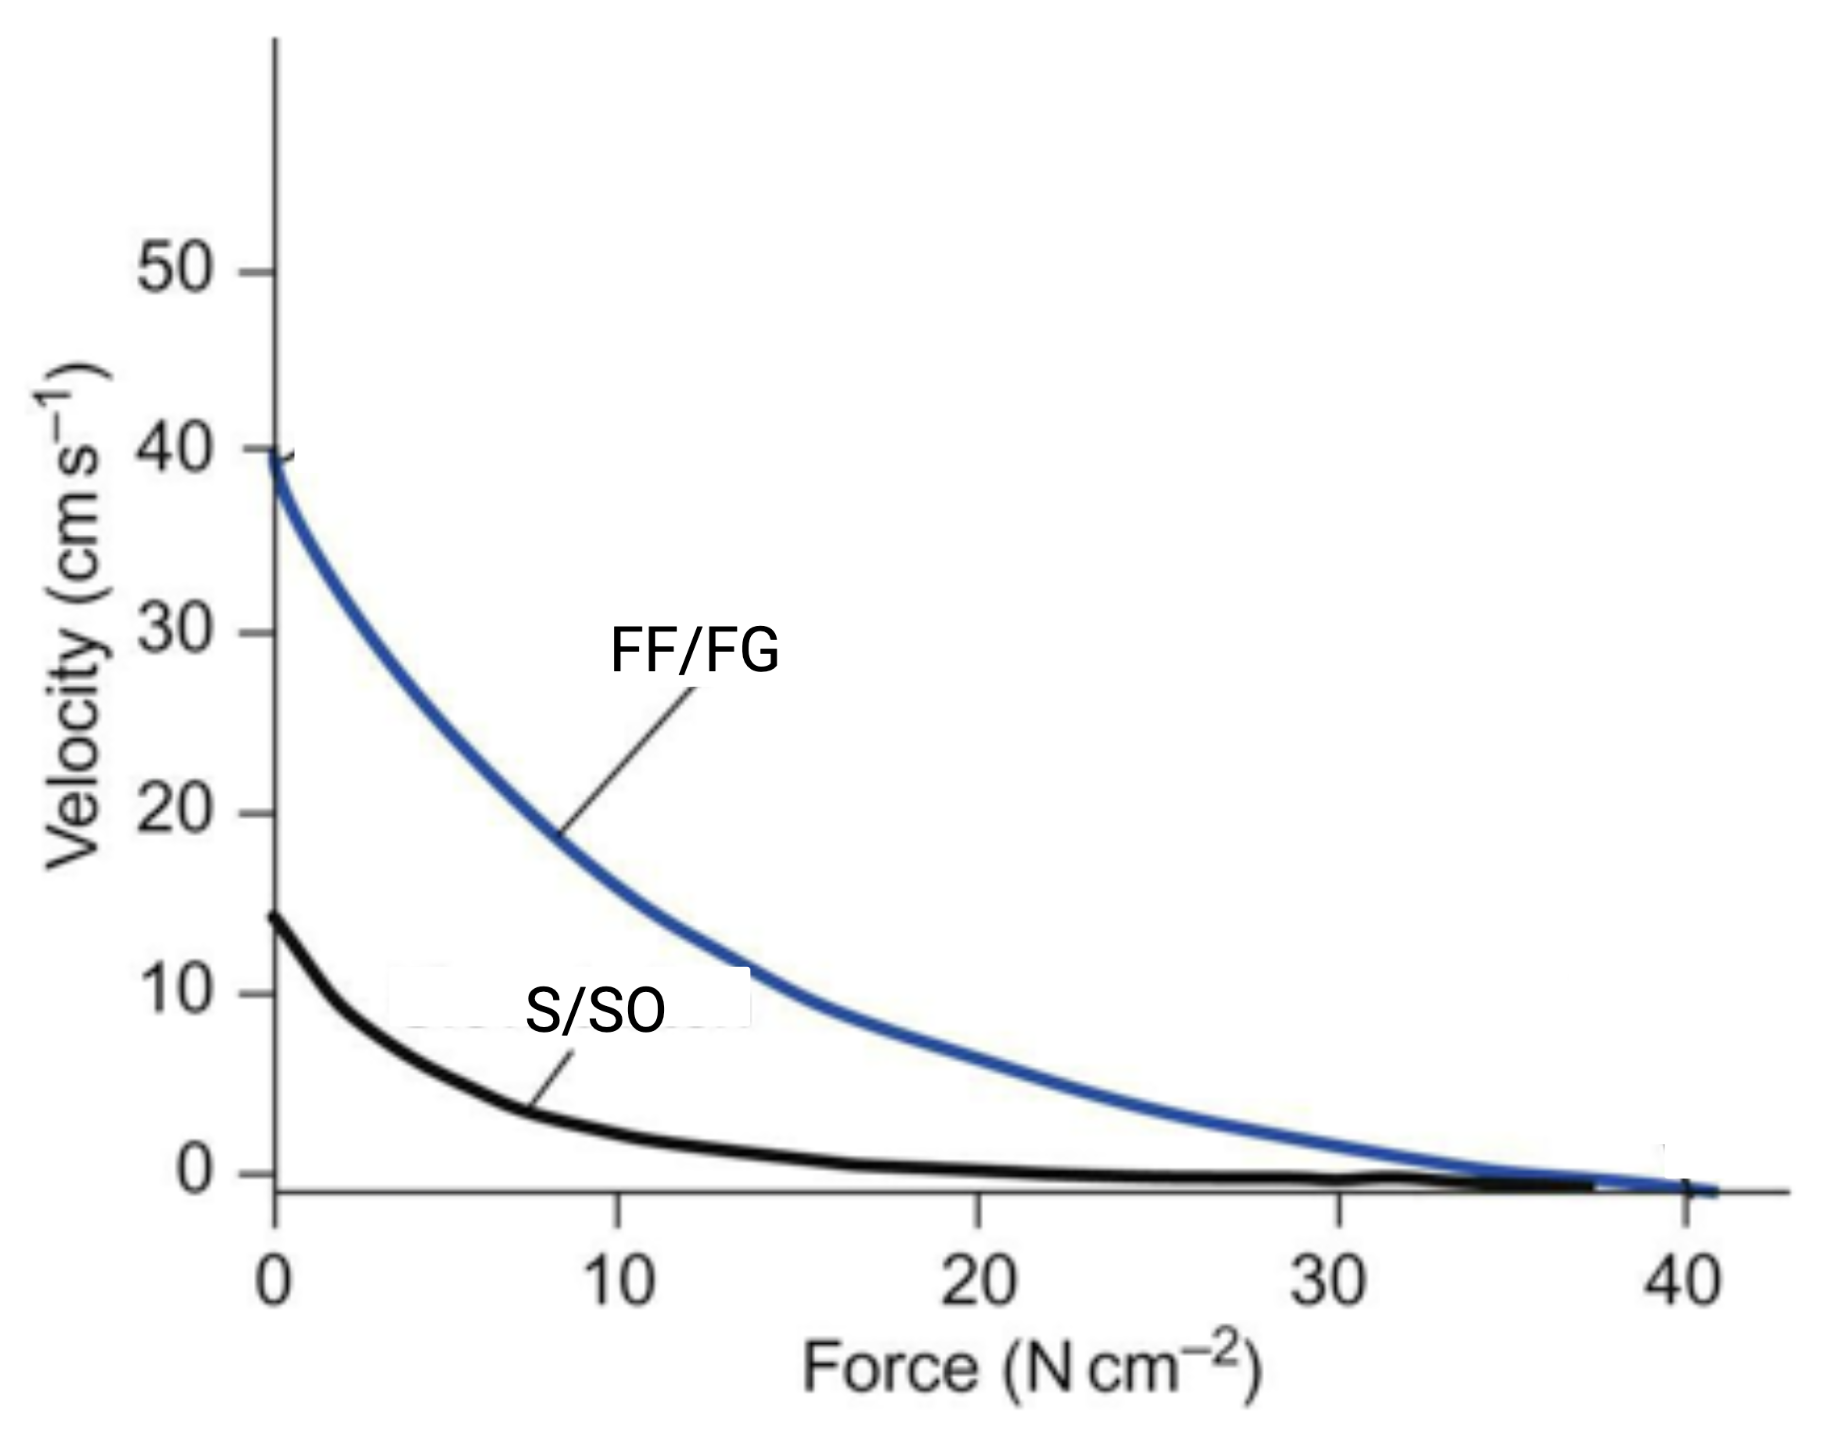
\includegraphics[width=1\linewidth]{./figure/fiber_type_FV.png}
    \caption{Force and Shortening Velocity of FF/FG and S/SO Motor Units \footnotesize{(Created in BioRender.com, Modified from \cite{feher_quantitative_2017})}}
    \label{fig:fiber_type_FV}
\end{figure}


\section{Motor Unit Twitch \& Tetany}

A single excitation of a muscle fiber produces enough activation to create a twitch, making a twitch the fundamental unit of active tension in the muscle fiber. The concept of a muscle fiber twitch is scaled up to a motor unit twitch. A muscle fiber twitch is the fundamental unit of active tension, a motor unit twitch is the fundamental unit of movement.\footnotemark\footnotetext{Just a note that by "unit" we don't mean unit as in a unit of measurement. Other words for how we are using the word unit may be "element" or "atom" or "particle".} Movements are created by muscle \textit{in situ}, and this means muscle fiber excitations and twitches occur in response to motor unit excitations, and the active tension developed by muscles that results in movement are based on motor unit twitches. Motor units have fidelity. When the neuron of a motor unit is excited all of the muscle fibers of the motor unit are excited. Recall from the data in Table \ref{table:Innervation_Ratios} that for the gastrocnemius this means a motor unit twitch includes approximately 1720 muscle fiber twitches. The fibers that are parallel increase the cross sectional area (A) and the tension.

\subsection{Motor Unit Type - Twitch \& Tetany Characteristics}

The three motor unit types display different twitch tension, twitch time and fatigue index (See Table \ref{table:Motor_Unit_Types}). These measurable functional characteristics are the result of the structural differences of both the motor unit neuron and the associated muscle fibers discussed in the previous section.

\begin{table}[h!]
\centering
\begin{tabular}{||c c c c||} 
 \hline
 Motor Unit Type & Twitch Tension & Twitch Time & Fatigue Index \\ [0.5ex] 
 \hline\hline
 Fast-Fatigable (FF)  & High & Fast & Low \\ 
 Fast-Resistant (FR)  & Moderate & Fast & Moderate \\
 Slow (S) &  Low & Slow & High \\ [1ex] 
 \hline
\end{tabular}
\caption{Motor Unit Types}
\label{table:Motor_Unit_Types}
\end{table}

\paragraph{Twitch Time}
Twitch time refers to the total time of the twitch with includes its upslope, time at peak or plateau, and time for downslope. A FF motor unit has a fast rise, short lived peak, and fast downslope. An S motor unit has a slower rise, longer plateau, and slower downslope. These characteristic curves (See Figure \ref{fig:mu_twitch}) contribute to the excitation frequency required for achieving tetany in the different motor unit types. An S motor unit can achieve tetany with an excitation frequency of 20-30 Hz since the twitches last longer and fuse (summate) more easily. A FF motor unit requires a higher frequency (80-100 Hz) to achieve tetany. 

\begin{figure}[!ht]
    \centering
    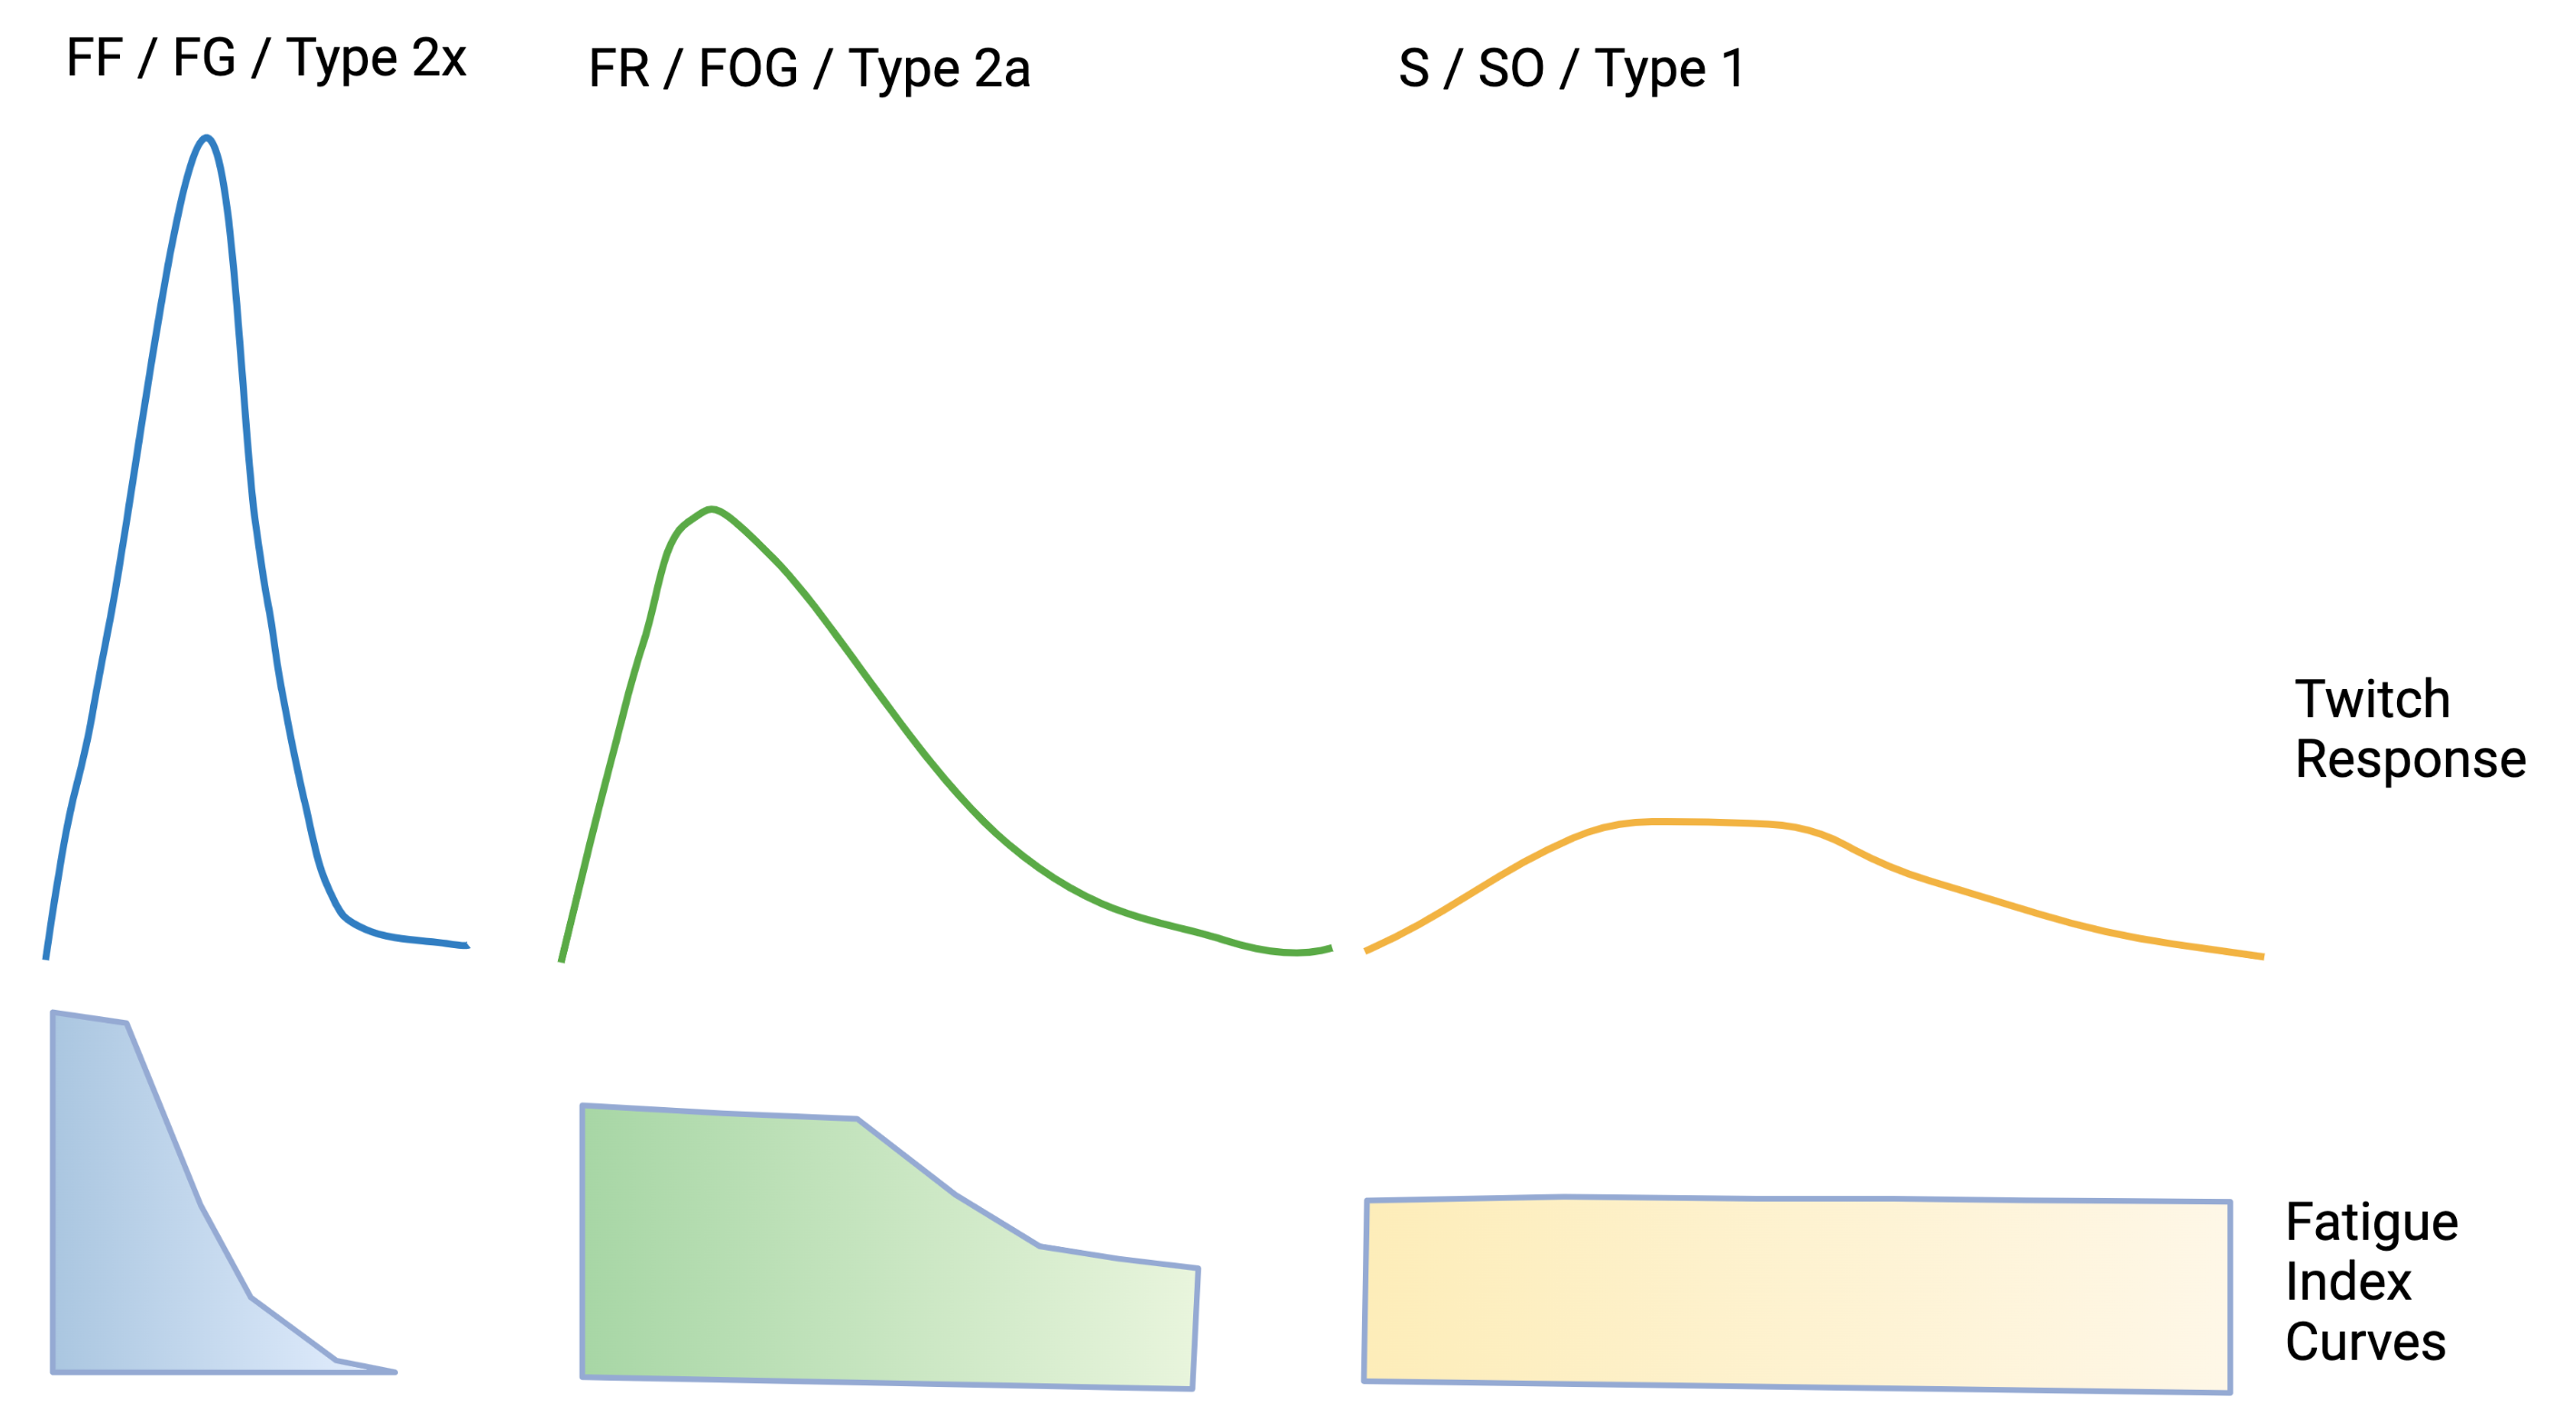
\includegraphics[width=1\linewidth]{./figure/mu_twitch.png}
    \caption{Motor Unit Twitch Characteristics \footnotesize{(Created in BioRender.com, Modified from \cite{jones_skeletal_2006}})}
    \label{fig:mu_twitch}
\end{figure}

\paragraph{Twitch Tension}
Twitch tension refers to the measurable force of a the tension developed during a twitch. Since tetany includes a summation of the twitches, a higher twitch tension results in a higher tetanic tension as well. Twitch tension is highest in the FF motor units for three reasons. First, these motor units have the highest number of muscle fibers (N, which is directly related to innervation ratio (IR)). Second, these motor units have, overall, a higher cross sectional area. Part of the larger cross area, but not all of it, is due to the higher number of fibers. The IR of a FF motor unit is approximately 2x higher than an S motor unit. However, the cross sectional area (A) is approximately 2.3x higher than an S motor unit \cite{bodine_maximal_1987, buchthal_motor_1980}. Third, these motor units have a slightly higher specific tension ($T_s$). Estimates are that the $T_s$ of FF motor units when tetanized is approximately $22 \ N \cdot cm^{-2}$ compared to S motor units approximately $17 \ N \cdot cm^{-2}$. Based on these estimates the $T_s$ of a FF motor unit is approximately 1.3x that of a S fiber. 

\paragraph{}

The tension of a motor unit twitch $T_{mu}$ is the sum of the motor units muscle fiber twitches $T_{mf}$. The equation:

\begin{equation}
    T_{mu} = N \cdot T_{mf} = N \cdot A \cdot T_s
\end{equation}

\begin{itemize}
    \item $N$ refers to the number of muscle fibers. This either is (for one motor unit) or can be estimated by (for an entire muscle) the innervation ratio.\footnotemark\footnotetext{$IR = \frac{N_{mf}}{N_{mu}}$ (Note, when there is one motor unit, $N = IR = N_{mf}$)}
    \item $A$ refers to the cross sectional area - an indication of how many sarcomeres are in parallel in the fiber.
    \item $T_s$ refers to the tension created for each unit of cross sectional area.
\end{itemize}

Using the above equation and estimates of FF motor units compared to S motor units we can derive an estimate of the FF motor unit $T_{mu}$ relative to the S motor unit. 

\paragraph{}
Assumptions:
\begin{itemize}
    \item FF motor unit IR, and therefore $N$ is 2x that of S motor units (more fibers)
    \item FF motor unit $A$ is 2.3x that of S motor units (greater cross sectional area)
    \item FF motor unit $T_s$ is 1.3x that of S motor units (higher tension per sarcomere)
\end{itemize}

An equation for the $T_{mu}$ for a FF compared to a S motor unit simply adjusts the variables based on a FF motor unit:

\begin{equation}
    T_{FF} = (N \cdot 2) \cdot (A \cdot 2.3) \cdot (T_s \cdot 1.3)
\end{equation}

This equation estimates that a FF motor unit can develop 6x more tension than an S motor unit. If based just on the number of fibers and the cross section area the estimate would be 4.6x. Therefore the number of fibers and the cross sectional area account for 76\% of the difference in tension between the FF and the S motor units. And the specific tension accounts for the remaining 24\%. Based on these estimates it is not surprising that differences in the specific tension between FF and S motor units is an area of controversy. When considering the likely variability between muscles, between samples, between mammalian species, differences as small as 1.3x are difficult to demonstrate \cite{lieber_skeletal_2010}. Some sources equate the $T_s$ between the two fiber types, $T_s \simeq 20 N \cdot cm^{-2}$ \cite{feher_quantitative_2017}, whereas others report them separately with albeit different estimates, FG $T_s \simeq 22 N \cdot cm^{-2}$, and SO $T_s \simeq 15 N \cdot cm^{-2}$ \cite{lieber_skeletal_2010}.

\paragraph{Fatigue Index}
Fatigue Index (FI) refers to how long tetany can be sustained for the FF, FR and S motor units. As Table \ref{table:Motor_Unit_Types} indicates, and Figure \ref{fig:mu_twitch} depicts the FF (fatigable) motor units have a low FI, whereas the S motor units have a high FI.

\subsection{Summary of Motor Unit Twitch \& Tetany}
The structural and functional differences between motor unit types result in expected differences in motor unit twitch and tetany characteristics. These differences lend themselves to the functional movement benefits of each type of motor units. FF motor units are optimized for fast, high force, high power - ballistic and temporary or intermittent movements. S motor units are optimized for slower, lower force and lower power - sustained, postural, stabilizing postures and movements. Further support of this story comes from how the motor units are recruited, that is, how tension is regulated.

\section{Active Tension Regulation}

Active tension is regulated through motor unit excitation. The two approaches include frequency summation (rate coding) of each motor unit and motor unit summation (recruitment) of more motor units. Both of these approaches start in the spinal cord with motor unit excitation.

\subsection{Motor Unit Excitation}

An $\alpha$-motor neuron, once excited, will release one neurotransmitter, ACh, at its axon terminal. ACh has one effect at the NMJ, creating excitatory micro-potentials on the motor end plate. In the CNS, more specifically for motor neurons in the spinal cord, competing neurotransmitters are released at synapses of the $\alpha$-motor neuron dendrites. The impact of these neurotransmitters can be excitatory or inhibitory. Since they occur after the synapse they are called excitatory post synaptic potentiations (EPSPs) or inhibitory post synaptic potentiations (IPSPs). Whether, and how frequently, an $\alpha$-motor neuron sends an excitation to the muscle fibers it innervates involves competition between the EPSPs and the IPSPs. For example, the IPSPs of certain protective reflexes associated with receptors in the muscle (see Golgi Tendon Organs below) can reduce the tension developed in a motor unit muscle fibers due to IPSPs lowering both the frequency of stimulation of a motor unit and the number of motor units recruited.

\subsection{Motor Unit Tetany - Frequency Summation}

Motor unit tetany involves the frequency of excitations. For any given motor unit, across all types, there is a range of excitation frequencies (rate coding) that can be used to vary the tension developed. It is estimated that frequency summation accounts for small fine tuning differences in tension. Frequency summation is not capable of resulting in large variations in tension in large part because it involves a set of muscle fibers that have a narrow functional frequency bandwidth. S type motor units can tetanize as low as 20 Hz, but don't develop any more force beyond perhaps 60 Hz (with a plateau occurring as low as 40 Hz). Similarly, FF motor units don't tetanize until they achieve upwards of 100 Hz and plateau at approximately 140-160 Hz. These differences, assuming linear increases in tension occur as frequency increases, represent a roughly 50\% increase in tension. If someone' grip strength is 100 pounds of force, then getting from 1 to 10 pounds of force requires a 10 times increase, getting from 1 to 100 pounds requires a 100 times increase. These increases in force cannot be accounted for by frequency summation. This has implications in situations discussed later which include a loss of motor units.

\paragraph{}

Frequency summation fine tunes and adjusts the tension in motor units but it is not capable of large fold changes in tension (or force). But, due to the role that excitation plays in motor unit tetany and the importance of tetany of motor unit muscle fibers for functional movements, the differences in the frequency of excitation to achieve tetany between the motor unit types is an important concept as we consider motor unit recruitment.

\subsection{Motor Unit Summation - Recruitment}

The primary way that muscle tension is regulated is through motor unit summation (recruitment). The recruitment of more motor units has the capability of greatly increasing the tension. From the example above, to go from 1 pound to a 100 pound hand grip requires the recruitment of few to perhaps all of the motor units involved in grip strength. Figure \ref{fig:Motor_unit_recruitment} depicts what happens when the three different motor units are recruited, first the SO fibers (S motor units), then the FOG fibers (FR motor units), and finally the FG fibers (FF motor units).\footnotemark\footnotetext{A future version of this figure will change upslope of these curves to represent the Twitch Time characteristics of the motor unit types).}


\begin{figure}[!ht]
    \centering
    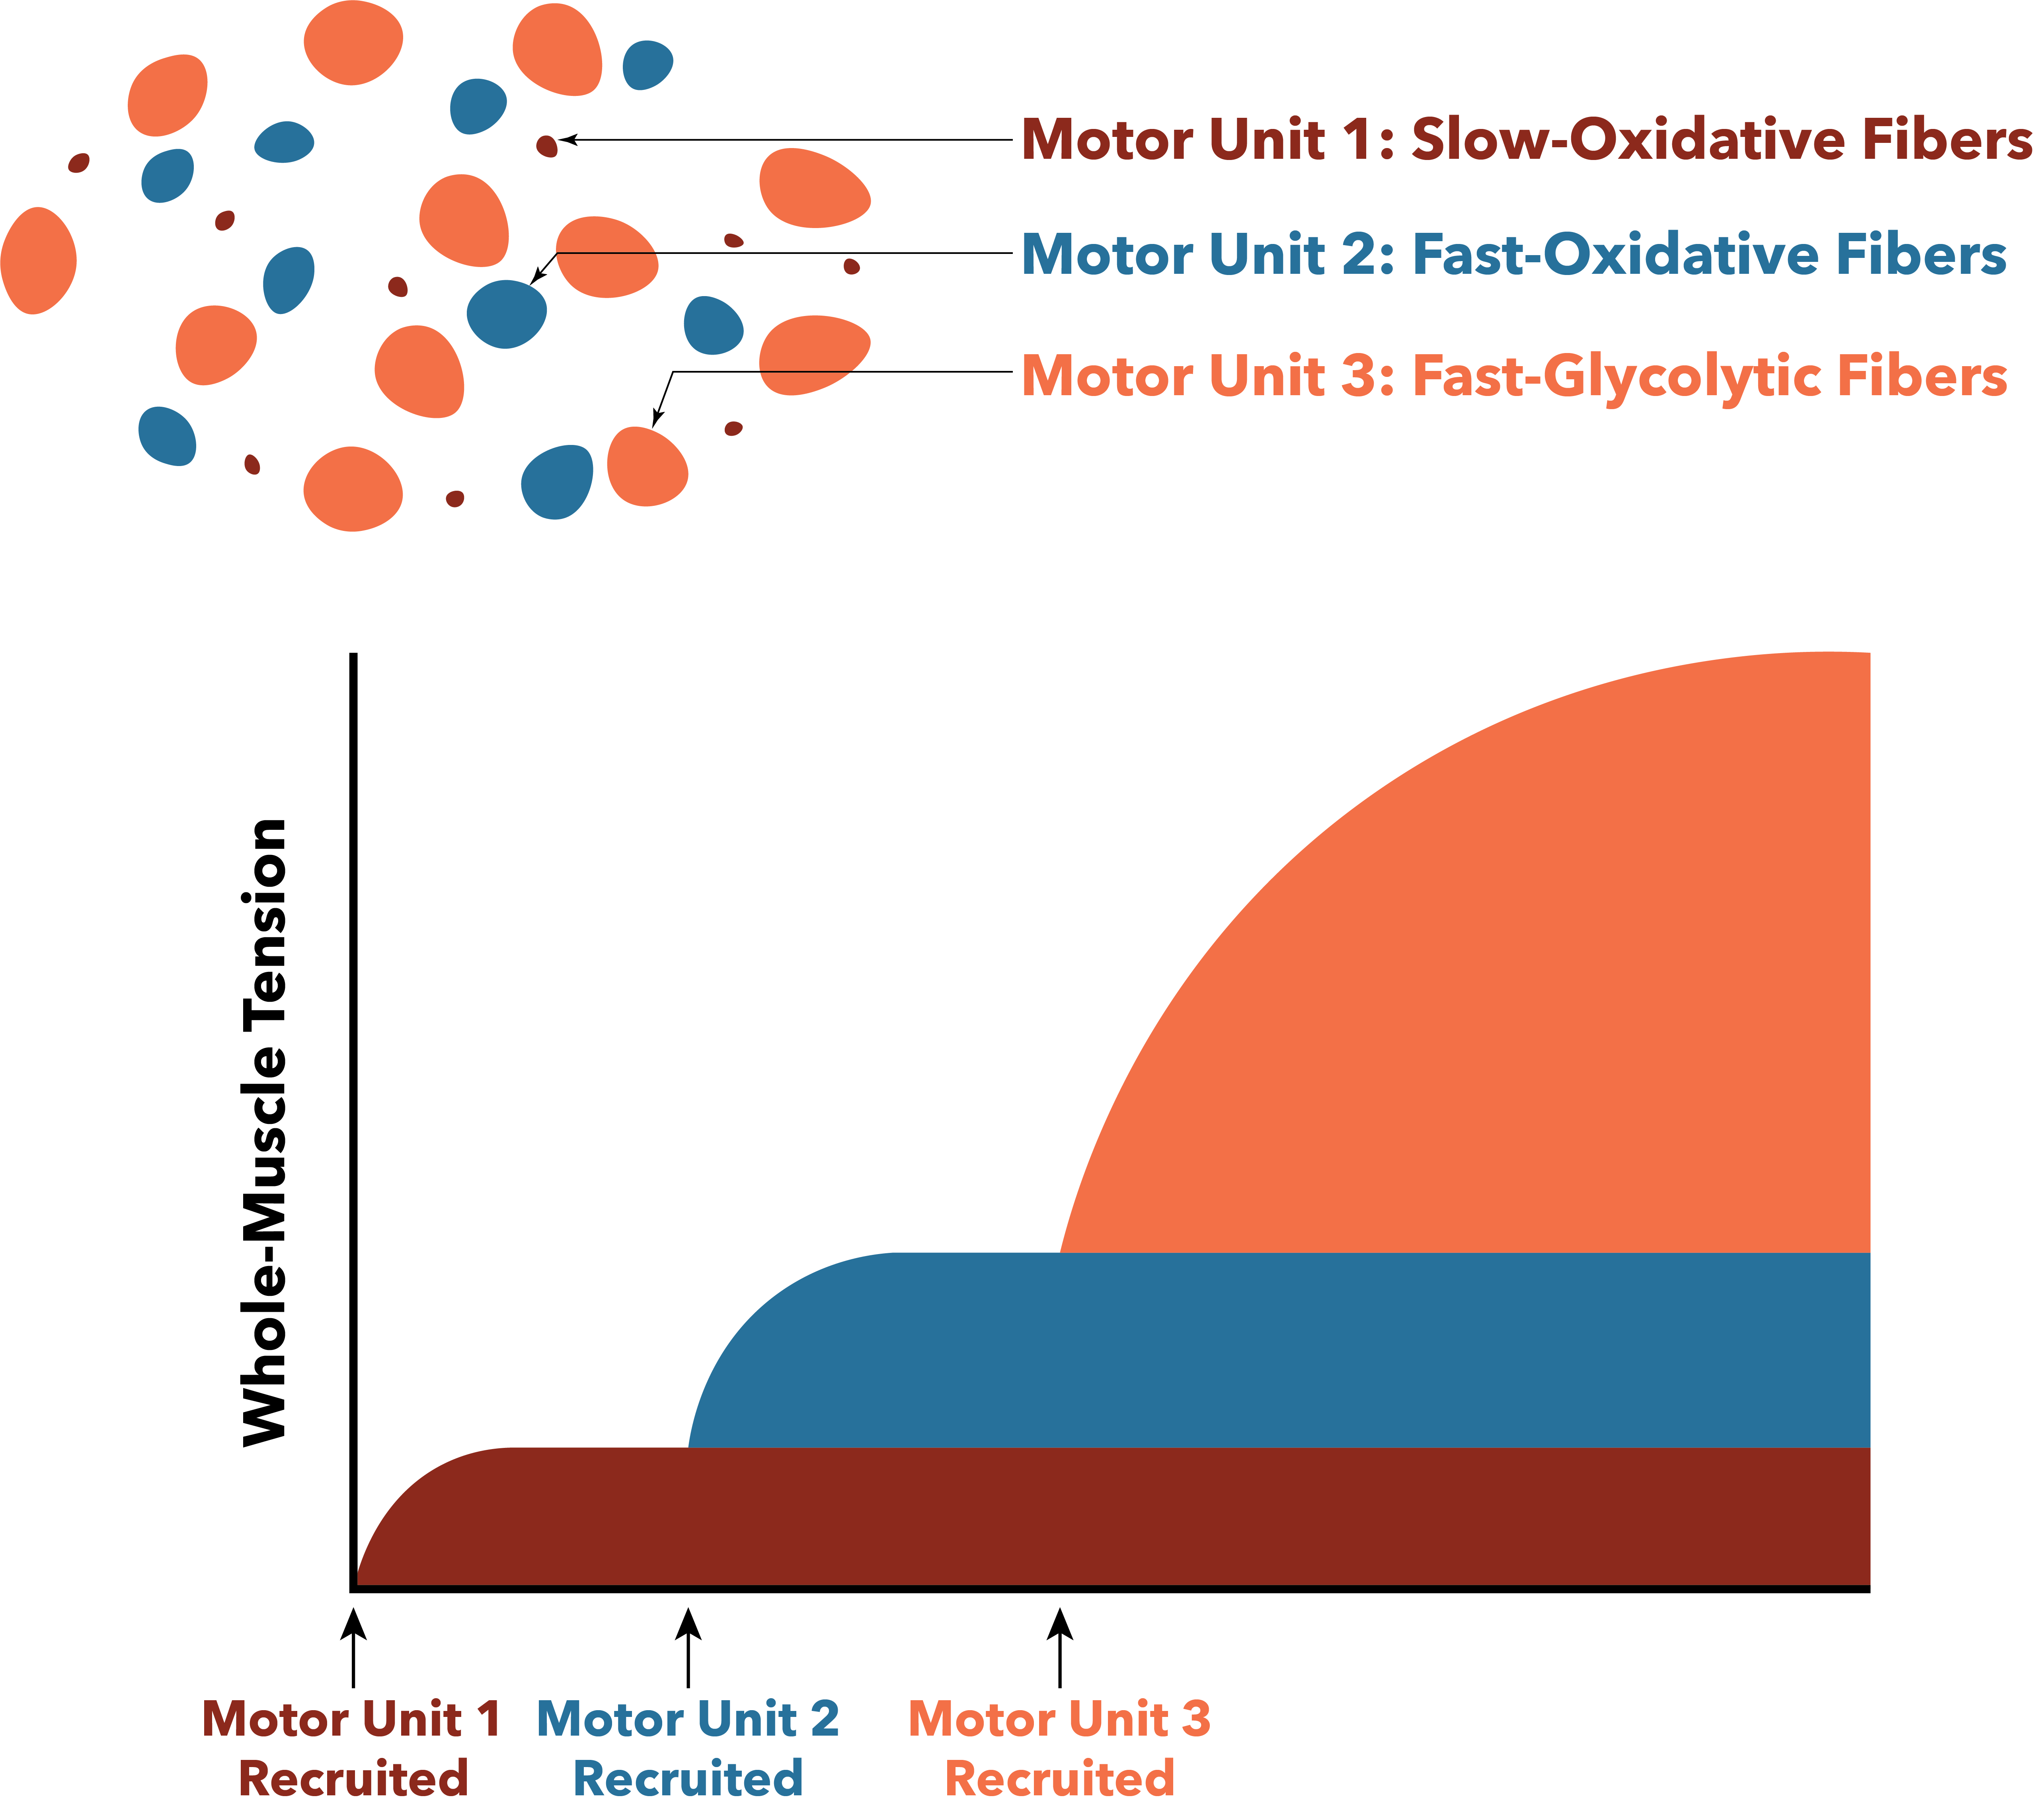
\includegraphics[width=1\linewidth]{./figure/Motor_unit_recruitment.png}
    \caption{Motor Unit Order of Recruitment \footnotesize{\href{https://commons.wikimedia.org/wiki/File:Motor_unit_recruitment.png}{Wikimedia Commons, CC BY 4.0})}}
    \label{fig:Motor_unit_recruitment}
\end{figure}

\paragraph{Size Principle of Motor Unit Recruitment}

The size principle of motor unit recruitment is based on the experimental observation that low tension requirements are met by first recruiting smaller motor units (S) with their associated SO fibers. As tension requirements increase the motor units recruited increase in size \cite{henneman_rank_1974}. This is due to two interrelated characteristics of the motor units themselves. First, smaller motor units require less excitation potentials to reach a membrane threshold potential. Lower CNS output into the region of the spinal cord (dorsal horn) with the dendrite pool of $\alpha$ motor neurons for a particular muscle first excites small dendrite membranes (they have less excitation inertia). As the CNS output increases in intensity, signaled as an increase in frequency of excitatory neurotransmitter impulses, there is an increase in excitation of the larger motor neurons. The second characteristic is that the larger motor neurons (FR and FF) require higher frequency excitations in order to achieve tetany.

\paragraph{Tension Developed during Motor Unit Summation - Recruitment}

Figure \ref{fig:n_motor_unit_recruitment} is a simulation based on the previously derived estimate that a FF motor unit generates 6x more tension than a S motor unit. This estimate accounts for the higher number of fibers, the greater cross sectional area of the fibers, and the greater specific tension of the fibers in an FF motor unit. Additional assumptions for this simulation include that the muscle has 100 motor units generating up to 100\% of of its maximal active tension; and that there are 20 S motor units, 20 S to FR transition motor units; 20 FR motor units; 20 FR to FF transition motor units; and 20 FF motor units. The S motor units each contribute 1 arbitrary unit (au) of tension, the FR motor units each contribute 3 au of tension, and the FF motor units each contribute 6 au of tension. The transition motor units are scaled linearly from 1 to 3, and from 3 to 6 in their respective transition zones. What is clear is that based on the order of recruitment (S to FF) there is an upward slope of tension with each new motor unit recruited. Jumps in tension as more motor units are recruited get larger as more motor units are recruited. Frequency summation tuning offers can further adjust these jumps. This tuning is more effective at lower tension with the small motor units since there are smaller jumps to accommodate.

\begin{figure}[!ht]
    \centering
    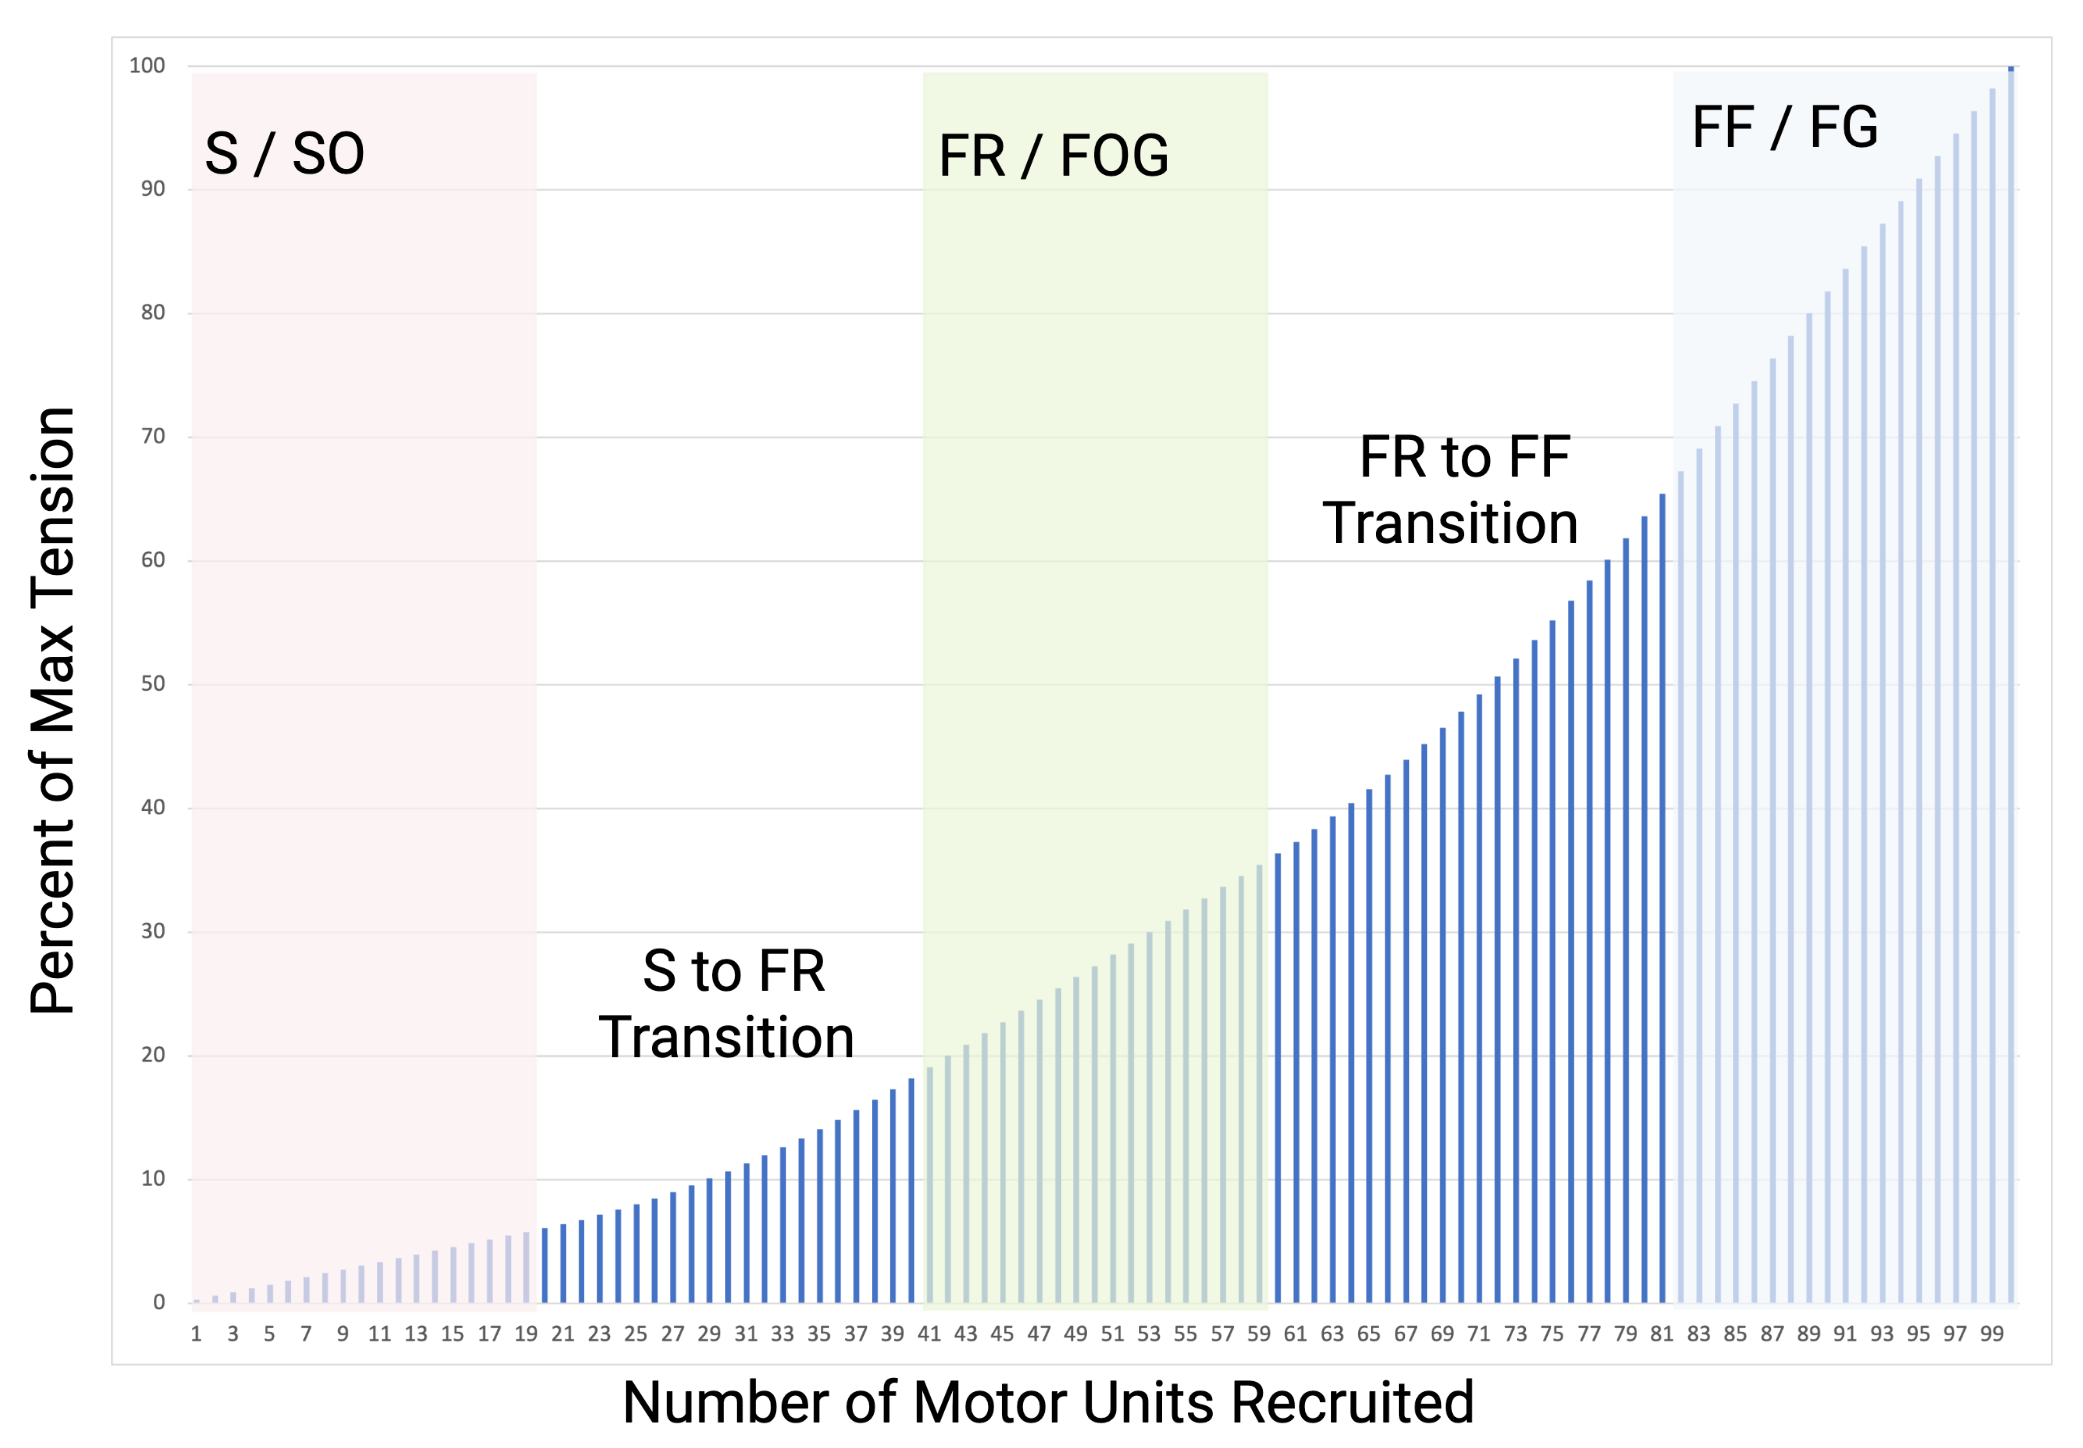
\includegraphics[width=1\linewidth]{./figure/n_motor_unit_recruitment.png}
    \caption{Simulation of Tension Developed during Motor Unit Summation - Recruitment (See text for simulation assumptions) \footnotesize{Created with Excel and BioRender.com})}
    \label{fig:n_motor_unit_recruitment}
\end{figure}

\paragraph{}

A commonly experienced consequence of the order of recruitment, that is clear in Figure \ref{fig:n_motor_unit_recruitment}, is that regardless of the muscle innervation ratio, there is less precision in tension regulation, and therefore less coordination and fine motor control when a muscle is being near maximal or maximally recruited. Muscles with lower IRs (such as the eye muscle described earlier with an IR of 5), will retain precision to a much higher level of tension, but it will still be reduced at higher tensions. If you have ever tried to fix your apple laptop and remove the small screws that require precision but a lot of force to remove, you understand the challenge of high tension precision.

\section{Regulatory Feedback}

It is estimated that between 40\% to 70\% of the nerves in a nerve bundle to a skeletal muscle fiber are $\alpha$-motor neurons (\underline{e}fferent nerves, \underline{e}xiting the spinal cord). The remaining axons are from sensor nerves (\underline{a}fferent nerves, \underline{a}ccessing the spinal cord). Regulation of tension is critically dependent on knowing whether the intention of tension is being met (whatever that intention may be) so that tension can be adjusted as necessary. Since neither motor control or neuroscience is a focus of this book (or course) this section is brief and focused on the muscle spindles and golgi tendon organs (GTOs) and how they influence tension regulation in the the spinal cord. 

\subsection{Muscle Spindles}

Muscle spindles are receptors that are excited when stretched and provide the central nervous system with information about muscle length and rate of stretching. With this information the muscle spindles are important contributors to proprioception (sensation and perception of position and movement). They are located within fascicles along side (parallel to) muscle fibers. It is conventional, once speaking of the muscle spindle, to refer to muscle fibers as extrafusal fibers (not part of the muscle spindle). The muscle spindles have both afferent and efferent innervation and their own small set of intrafusal contractile fibers. The intrafusal fibers are innervated by $\gamma$-motor neurons and allow the muscle spindle to adjust to the length of the muscle to remain sensitive to changes in length (See Figure \ref{fig:MuscleSpindle}). 

\begin{figure}[!ht]
    \centering
    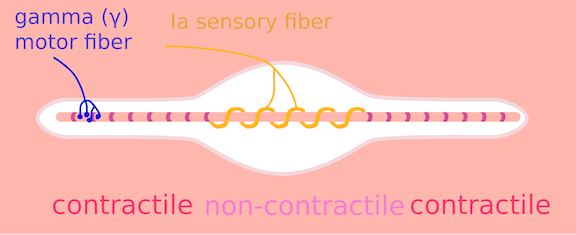
\includegraphics[width=1\linewidth]{./figure/MuscleSpindle.png}
    \caption{Muscle Spindle \footnotesize{\href{https://commons.wikimedia.org/wiki/File:MuscleSpindle.svg}{Wikimedia Commons, CC BY 4.0})}}
    \label{fig:MuscleSpindle}
\end{figure}

Afferent signals from the muscle spindles terminate at the spinal cord as well as higher up in the central nervous system for long loop reflexes and coordination (cerebellum) and the cerebral cortex (proprioception). The response of muscle spindles to a rapid increase in length (quick stretch) signals the dendrites of the $\alpha$-motor neurons of the agonist (same muscle that is being stretched) with excitatory post synaptic potentiations (EPSPs); and the dendrites of the $\alpha$-motor neurons of the antagonist (opposite muscles of those that are being stretched) with inhibitory post synaptic potentiations (IPSPs). Collectively these actions are referred to as the stretch reflex. If the stretch is quick enough and excites enough muscle spindles the EPSPs are sufficient to excite $\alpha$-motor neurons which provoke muscle excitation and activation. Testing stretch reflexes is an important component of a physical exam when the integrity of the $\alpha$-motor neuron, or any part of the sensory - motor reflex loop, is in question.

\subsection{Golgi Tendon Organs}

Golgi tendon organs (GTOs) are on the mostly tendon side of the transition space known as the musculotendinous junction. They are so close to muscle fibers that each GTO is connected in series with 5-20 muscle fibers. In this position the GTOs detect tension in muscle and tendinous fibers \cite{macefield_physiological_2005}. The GTO is excited by tension within the muscle fibers or tendon. Afferent impulses from the GTOs terminate in the spinal cord and cerebellum. GTO afferents in the spinal cord result in IPSPs of the agonist muscle. Inhibiting the agonist limits active tension as a protective mechanism.

\section{\textit{Clinical Physiology Connections}}

\subsection{Electromyogram (EMG)}

Each time a muscle fiber is activated it is caused by an excitation (action potential) from the nerve to the motor end plate, and along the sarcolemma of all the fibers that are innervated by that $\alpha$-motor neuron. Therefore, each muscle fiber activation is associated with an electrical signal. An EMG electrode near the fiber can record this electrical activity. The electrode can either be a small needle that acts as an antenna to record local electrical activity or a surface electrode (sEMG). If using a needle, the raw EMG signal can be used to accurately determine when a particular muscle is active (regardless of depth or size of the muscle). sEMG can be used to determine when a particular muscle is active when the muscle of interest is superficial and large enough to avoid cross talk at the sEMG electrode, but cannot be accurately used to determine specific activation of deep or small muscles. For example, sEMG just lateral to the spine cannot be expected to accurately identify activation of deep muscles such as the multifidi.

\paragraph{EMG quantification} It is difficult to quantify the activity of a muscle from a raw EMG signal. The EMG contains electrical signals from every muscle fiber in the vicinity of the EMG electrode which creates a very noisy signal (See Figure \ref{fig:EMG_ARV}). From the raw signal the Average Rectified Voltage (ARV) EMG can be computed. ARV is a time-windowed mean of the absolute value of the signal (turns all voltages into positive values). ARV is useful for further analysis such as recording the excitation patterns of a muscles that may include changes in excitation or as the first step towards more advanced analyses \cite{merletti_surface_2016}. The relationship between EMG activity and muscle tension is most valuable during isometric activation because the association between activation and tension changes with changes in length (length-tension relationship), and with different velocities (force-velocity relationship).

\begin{figure}[!ht]
    \centering
    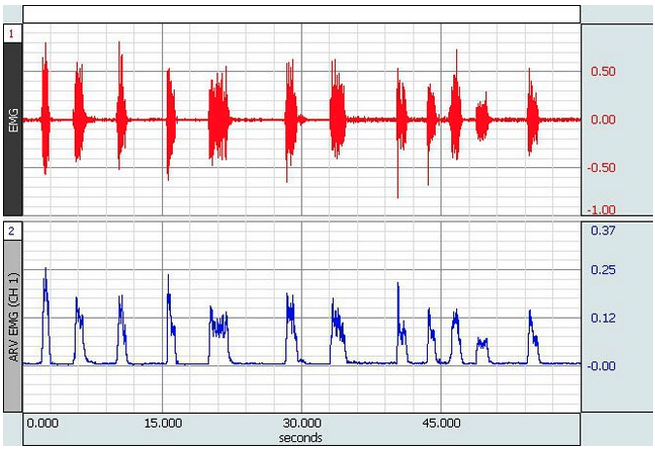
\includegraphics[width=1\linewidth]{./figure/EMG_ARV.png}
    \caption{Raw (upper) and ARV (lower) EMG Signals \footnotesize{Data collected using Biopaq acquisition hardware and Acknowledge software in the author's lab (SC)}}
    \label{fig:EMG_ARV}
\end{figure}

\paragraph{Biofeedback}

sEMG is a valuable form of biofeedback to indicate that a certain muscle has been activated. Commercially available devices provide visual or auditory signals so a patient can learn to activate a muscle. Common applications of the EMG for biofeedback is activation in the vastus medialis after anterior cruciate ligament surgery, or the lower trapezius during shoulder flexion or abduction.

\paragraph{Motor Unit Number and Size Indices (MUNIX \& MUSIX)}

The motor unit number index (MUNIX) and the motor unit size index (MUSIX) are based on sEMG data interpreted through a mathematical model to estimate an index of the number and size of functional $\alpha$-motor neurons for a muscle \cite{nandedkar_motor_2004}. MUNIX is not an absolute count of motor units, and MUSIX is not an absolute size of the motor units. But they do provide an estimate that correlates with other measures and they have reasonable reliability. Considering the test only takes 3-5 minutes per muscle, is non-invasive and relatively comfortable (as compared to other approaches), they have gained popularity in clinical neurology and neurophysiology. MUNIX is considered an effective bio-marker for assessing disease progression and an alternative clinical trial outcome for conditions associated with a decrease in motor units such as amyotrophic lateral sclerosis (ALS). It has also been proposed for use in the evaluation of peripheral neuropathies, particularly in demyelinating neuropathies with conduction block. While there have been less studies, MUNIX is starting to be evaluated in a variety of central nervous system disorders (such as spinal cord injury, stroke, and cerebral palsy \cite{fatehi_utility_2018}. 

A study of healthy individuals between 20 and 80 years of age demonstrated a reduction in MUNIX and MUSIX values with aging, particularly over the age of 60, indicating that they may be valuable biomarkers for research on the prevention and treatment of sarcopenia \cite{cao_reference_2020}. Sarcopenia is an age-related progressive loss of muscle mass and strength \cite{dao_sarcopenia_2020}. It is a type of muscle atrophy primarily caused by the aging process and certainly confounded by physical inactivity and malnutrition. Sarcopenia tends to result in a larger loss of FF motor units and FG (Type 2a) muscle fibers. If a loss of motor units is inevitable with aging, then healthy aging would strive for lifestyles that promote increasing MUSIX despite an inevitable decline in MUNIX. A consequence of this shift (reduced MUNIX and increased MUSIX) would be a reduction in muscle tension regulation. Therefore, the choice of lifestyle would need to consider the motor control (balance, coordination) capabilities in such individuals.

\subsection{Nerve Conduction Velocity (NCV)}

Nerve conduction velocity (NCV) refers to the time it takes for an excitation to travel a certain distance. It can be measured clinical with electrodiagnostic testing that includes EMG. A stimulus is presented proximally at a peripheral nerve and the distal muscle excitation (via EMG) or axonal excitation is measured.

The tight regulation of active tension for coordinated movement requires fidelity in the signals coming from the central nervous system.\footnotemark\footnotetext{Fidelity in this context means that intended signals are accurately sent where and when they are requested.} If the myelin sheath of an $\alpha$-motor neuron is damaged the NCV is reduced. If the NCV is reduced then the ability to activate muscles with high fidelity signals is impaired resulting in delays in the generation of active tension, limiting the ability to increase active tension when needed. These changes occur for two reasons, first, limitations in frequency summation, and second, limitations in motor unit summation. This is precisely what happens in peripheral demyelinating diseases such as Guillain-Barre syndrome, Chronic Inflammatory Demyelinating Polyradiculoneuropathy, and Anti-Myelin Associated Glycoprotein Neuropathy. The demyelinating disease known as Multiple Sclerosis (MS) also impairs signal fidelity, however, it is a central nervous system condition. Therefore, in MS the loss of signal fidelity does not directly alter the peripheral NCV, it impairs central NCV which interrupts signals that excite the motor unit dendrites in the spinal cord which contributes to a more complicated, nuanced and variable clinical presentation in terms of the impact it can have on motor function such as coordination.


\section{Summary \& Next Step}

Motor units connect the central nervous system to muscle fibers. Varying the frequency of excitation and the number of motor units excited allows the CNS to vary the active tension provided by a muscle. Tight regulation of this active tension is required for motor control. There are three accepted classifications of motor units and they correspond to three accepted accepted classifications of muscle fibers. The structural characteristics of these motor units and muscle fibers are related to distinct functional characteristics in twitch and tetany. Recruitment of motor units is the primary mechanism for varying tension with variations in the frequency of excitation providing a small range of tension variation that allows for fine tuning the nearly continuous range of possible tensions. Muscle spindles and golgi tendon organs provide the CNS with feedback about muscle tension, stretch and length. EMG can capture valuable information about motor unit and muscle excitation as well as the determination of NCV. The next chapter expands on the metabolic characteristics of muscle fibers and the impact muscle energetics has on function as well as the demands that muscle energetics places on other body systems.

\printbibliography[heading=subbibintoc]